
%(BEGIN_QUESTION)
% Copyright 2011, Tony R. Kuphaldt, released under the Creative Commons Attribution License (v 1.0)
% This means you may do almost anything with this work of mine, so long as you give me proper credit

According to the operator, this pressure-control system is not regulating filter water pressure correctly.  The controller faceplate indicates the pressure holding at setpoint (110 PSI), but pressure indicated by a pressure gauge on the outlet pipe of the filter shows substantially less pressure (85 PSI):

$$\includegraphics[width=15.5cm]{i03284x01.eps}$$

Your first test is to measure loop current in the circuit connecting the pressure transmitter to the pressure controller.  There, your multimeter registers 15.7 milliamps.

\vskip 10pt

Identify the likelihood of each specified fault for this control system.  Consider each fault one at a time (i.e. no coincidental faults), determining whether or not each fault could independently account for {\it all} measurements and symptoms in this circuit.

% No blank lines allowed between lines of an \halign structure!
% I use comments (%) instead, so that TeX doesn't choke.

$$\vbox{\offinterlineskip
\halign{\strut
\vrule \quad\hfil # \ \hfil & 
\vrule \quad\hfil # \ \hfil & 
\vrule \quad\hfil # \ \hfil \vrule \cr
\noalign{\hrule}
%
% First row
{\bf Fault} & {\bf Possible} & {\bf Impossible} \cr
%
\noalign{\hrule}
%
% Another row
PT out of calibration (outputting wrong current) &  &  \cr
%
\noalign{\hrule}
%
% Another row
PIC input out of calibration (not interpreting PV signal properly) &  &  \cr
%
\noalign{\hrule}
%
% Another row
PIC output out of calibration (not sending correct mA signal to I/P) &  &  \cr
%
\noalign{\hrule}
%
% Another row
Pressure gauge out of calibration (not displaying pressure properly) &  &  \cr
%
\noalign{\hrule}
%
% Another row
I/P out of calibration (not outputting correct pressure) &  &  \cr
%
\noalign{\hrule}
%
% Another row
Control valve is oversized &  &  \cr
%
\noalign{\hrule}
%
% Another row
Control valve is undersized &  &  \cr
%
\noalign{\hrule}
%
% Another row
PIC is poorly tuned (not making good control ``decisions'') &  &  \cr
%
\noalign{\hrule}
%
% Another row
Instrument air supply not at full pressure &  &  \cr
%
\noalign{\hrule}
} % End of \halign 
}$$ % End of \vbox

\underbar{file i03284}
%(END_QUESTION)





%(BEGIN_ANSWER)

This is a graded question -- no answers or hints given!

%(END_ANSWER)





%(BEGIN_NOTES)

A good diagnostic principle to apply here is that of {\it correspondence}: check for which variables properly correspond with each other, and which do not.  Clearly, the 110 PSI registered by the controller does not correspond with the 85 PSI registered by the pressure gauge, but this alone does not tell us where the problem lies.

If we take the measured milliamp signal (15.7 mA) and convert that into a corresponding pressure given the transmitter's range of 0 to 150 PSI, we may compare this calculated pressure value against the controller's display and the gauge's display to see which one agrees.  In this case, 15.7 mA is equivalent to 109.69 PSI, which closely agrees with the controller display but not with the gauge.

From this we may conclude that the controller is not at fault, because it is receiving a current signal equivalent to 110 PSI and that is what it is displaying.  Either the problem must lie with the transmitter (i.e. the real pressure is 85 PSI but the transmitter is incorrectly outputting a signal saying the pressure is 110 PSI), or it must lie with the gauge (i.e. the real pressure is 110 PSI and the gauge simply isn't reading right).

% No blank lines allowed between lines of an \halign structure!
% I use comments (%) instead, so that TeX doesn't choke.

$$\vbox{\offinterlineskip
\halign{\strut
\vrule \quad\hfil # \ \hfil & 
\vrule \quad\hfil # \ \hfil & 
\vrule \quad\hfil # \ \hfil \vrule \cr
\noalign{\hrule}
%
% First row
{\bf Fault} & {\bf Possible} & {\bf Impossible} \cr
%
\noalign{\hrule}
%
% Another row
PT out of calibration (outputting wrong current) & $\surd$ &  \cr
%
\noalign{\hrule}
%
% Another row
PIC input out of calibration (not interpreting PV signal properly) &  & $\surd$ \cr
%
\noalign{\hrule}
%
% Another row
PIC output out of calibration (not sending correct mA signal to I/P) &  & $\surd$ \cr
%
\noalign{\hrule}
%
% Another row
Pressure gauge out of calibration (not displaying pressure properly) & $\surd$ &  \cr
%
\noalign{\hrule}
%
% Another row
I/P out of calibration (not outputting correct pressure) &  & $\surd$ \cr
%
\noalign{\hrule}
%
% Another row
Control valve is oversized &  & $\surd$ \cr
%
\noalign{\hrule}
%
% Another row
Control valve is undersized &  & $\surd$ \cr
%
\noalign{\hrule}
%
% Another row
PIC is poorly tuned (not making good control ``decisions'') &  & $\surd$ \cr
%
\noalign{\hrule}
%
% Another row
Instrument air supply not at full pressure &  & $\surd$ \cr
%
\noalign{\hrule}
} % End of \halign 
}$$ % End of \vbox

%INDEX% Basics, control loop troubleshooting: determining cause of control problem

%(END_NOTES)


